\begin{frame}{Commercial examples of the use of mAb}
    \begin{block}{Trastuzumab against HER2-positive breast cancer}
        \vspace{1em}
        \begin{minipage}{0.495\textwidth}
            \begin{figure}
                \centering
                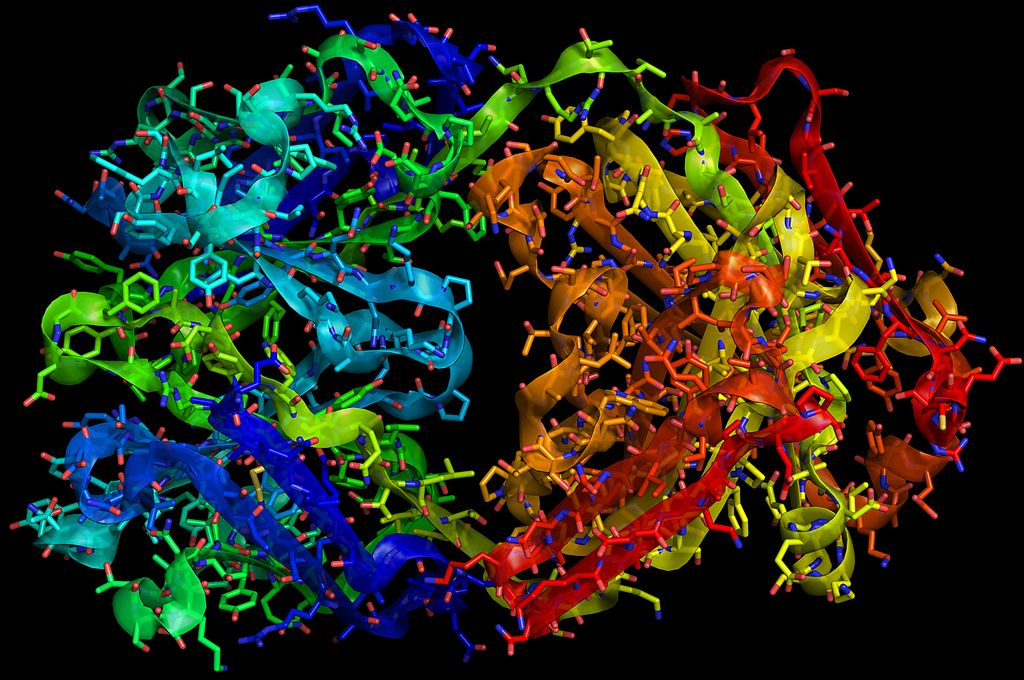
\includegraphics[width=\textwidth]{../Images/herceptin.jpg}
            \end{figure}  
        \end{minipage}\hfill
        \begin{minipage}{0.495\textwidth}
            \begin{figure}
                \centering
                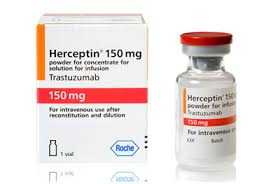
\includegraphics[width=\textwidth]{../Images/trastuzumab.jpg}
            \end{figure}    
        \end{minipage}
    \end{block}
\end{frame}

\begin{frame}{Commercial examples of the use of mAb}
    \begin{block}{Trastuzumab against HER2-positive breast cancer}
        % \vspace{1em}
        
        \begin{exampleblock}{Action mechanism}
            \begin{itemize}
                \item In the cancer cells, the HER2 protein is over-expressed
                \item The HER2 protein is a transmembrane protein, which then
                        proliferates along with the cancer cells
                \item Trastuzumab blocks HER2 activation and dimerization 
                \item The mAb also induces ADCC (Antibody Dependent Cell Cytotoxicity)
            \end{itemize}
        \end{exampleblock}

        \begin{exampleblock}{Treatment characteristics}
            \begin{itemize}
                \item 1-year long chemotherapy
                \item One injection every 3 weeks ($6$ mg/kg dose)
                \item Cost per patient : $17000$ €
            \end{itemize}
        \end{exampleblock}
    \end{block}

\end{frame}

\begin{frame}{Commercial examples of the use of mAb}
    \begin{block}{Trastuzumab against HER2-positive breast cancer}
        \begin{figure}
            \centering
            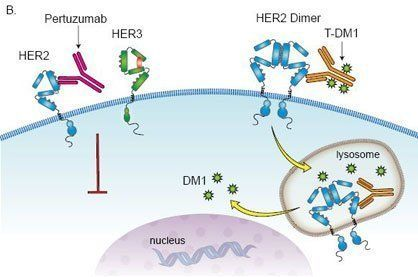
\includegraphics[width=0.8\textwidth]{../Images/her2_pertuzumab.jpg}
            \caption{HER2 dimerization and treatment by trastuzumab}
        \end{figure}
    \end{block}
\end{frame}


\begin{frame}{Commercial examples of the use of mAb}
    \begin{block}{Rituximab against lymphoma and leukemia}
        \vspace{1em}
        \begin{minipage}{0.495\textwidth}
            \begin{figure}
                \centering
                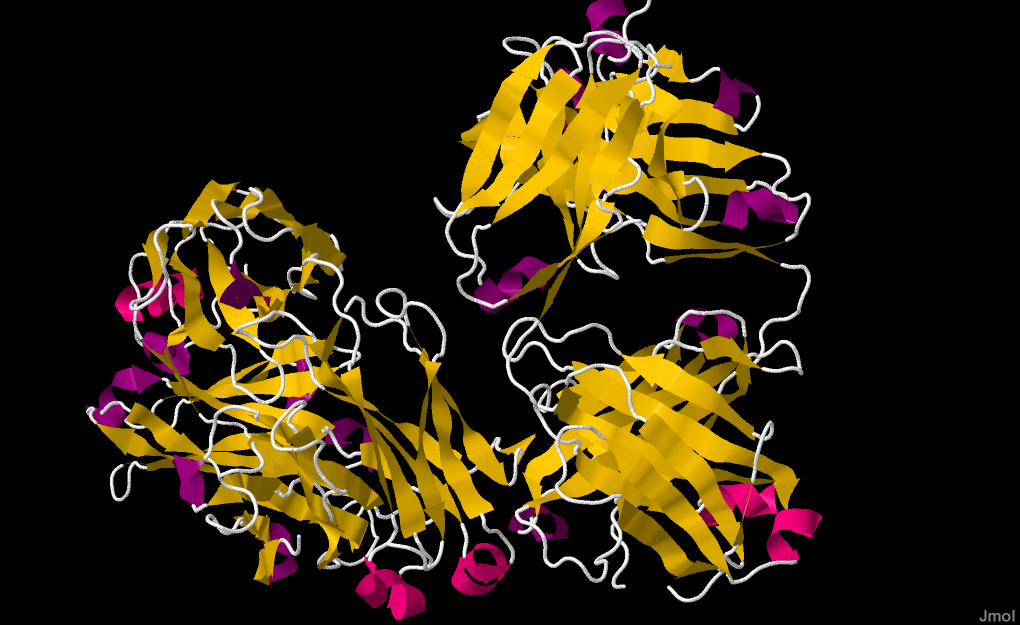
\includegraphics[width=\textwidth]{../Images/Rituximab.png}
            \end{figure}  
        \end{minipage}\hfill
        \begin{minipage}{0.495\textwidth}
            \begin{figure}
                \centering
                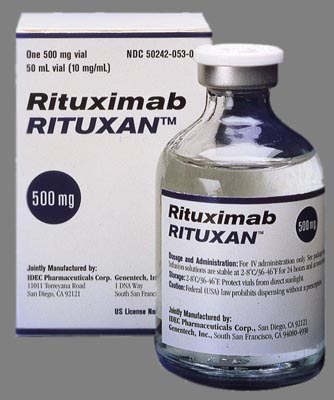
\includegraphics[width=0.8\textwidth]{../Images/rituxan.jpg}
            \end{figure}    
        \end{minipage}
    \end{block}
\end{frame}

\begin{frame}{Commercial examples of the use of mAb}
    \begin{block}{Rituximab against lymphoma and leukemia}
        \begin{exampleblock}{Action mechanism}
            \begin{itemize}
                \item In a lymphoma, cells born in the lymphatic system proliferate
                \item The rituximab Fab fragment binds to B-cells' CD20 antigen
                \item Multiple toxicity pathways are then induced
            \end{itemize}
        \end{exampleblock}
        
        \begin{exampleblock}{Treatment economics}
            \begin{itemize}
                \item One of the top 20-selling drugs in the world
                \item 2020 sales : $4,52$ billion \$, sold by Roche
            \end{itemize}
        \end{exampleblock}
    \end{block}
\end{frame}

